% in this file I leave the figure captions outside\ caption{} because I want them
% to be formatted in the same way as the general text (double spaced and linenumbered)
\captionsetup[figure]{labelfont={sc},labelformat={default},labelsep=period,name={Supplementary Figure}}

%%%%%%%%%%%%%%%%%%%%%%%%%%%%%%%%%%%%%%%%%%%%%%%%%%%%%%%%%%%%%%%%%%
%%%%%%%%%%%%%%%%    FIGURE CROSS VALIDATION    %%%%%%%%%%%%%%%%%%%
%%%%%%%%%%%%%%%%%%%%%%%%%%%%%%%%%%%%%%%%%%%%%%%%%%%%%%%%%%%%%%%%%%

\begin{figure}[!h]
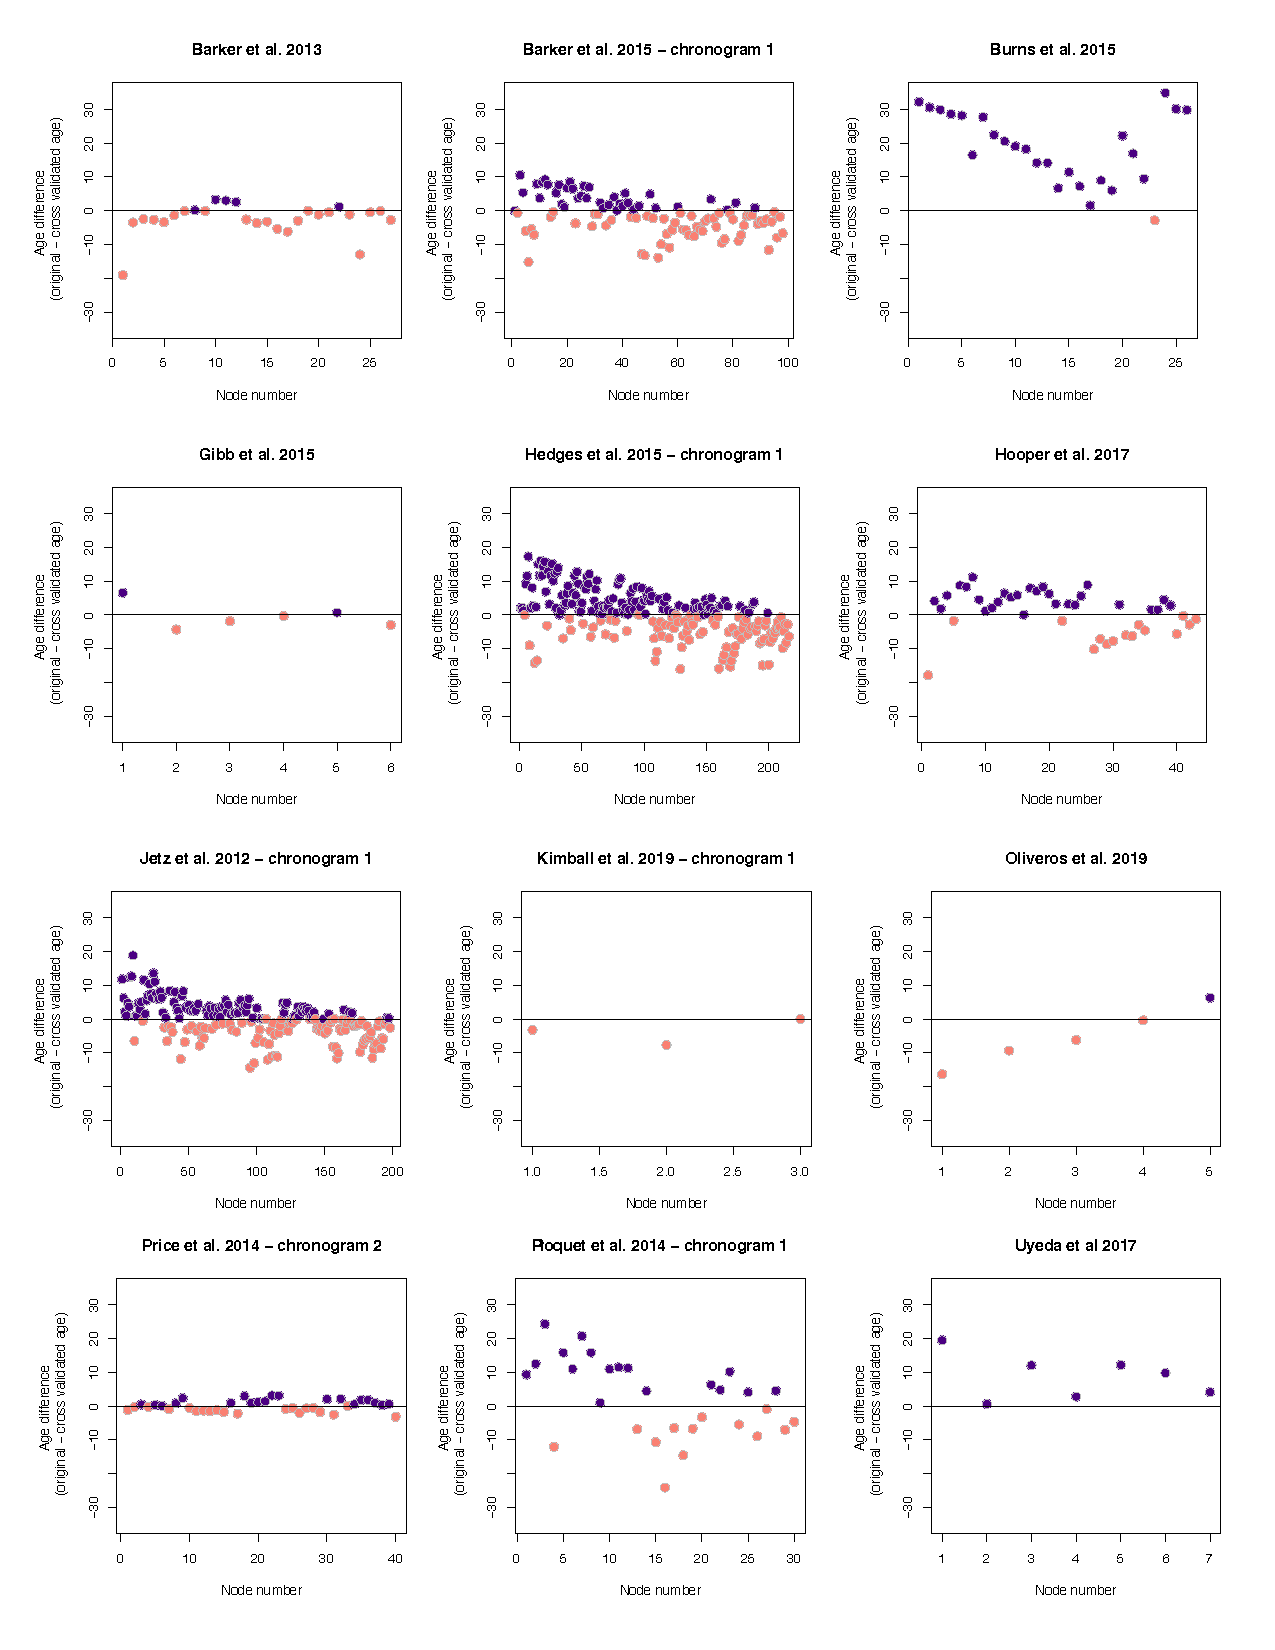
\includegraphics{../figures/figure-cross-validation/fig-cross-validation-xy-plots-diffs.pdf}
\caption{Results from cross validation analysis. Each plot shows the difference between the original age estimated and those obtained with a DateLife analysis, per node.}
\label{fig:cvXYdiffs}
\end{figure}

%%%%%%%%%%%%%%%%%%%%%%%%%%%%%%%%%%%%%%%%%%%%%%%%%%%%%%%%%%%%%%%%%%
%%%%%%%%%%%%%%%%   CROSS VALIDATION CHRONOGRAMS   %%%%%%%%%%%%%%%%
%%%%%%%%%%%%%%%%%%%%%%%%%%%%%%%%%%%%%%%%%%%%%%%%%%%%%%%%%%%%%%%%%%

\begin{figure}[!h]
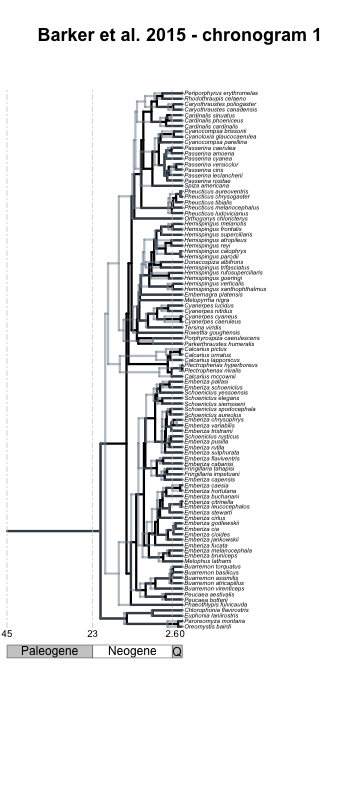
\includegraphics{../figures/figure-cross-validation/cross_validation_2.png}
\caption{Cross validation of Barker et al. (\protect\hyperlink{ref-barker2015new}{2015}) chronogram 1. The chronogram shown in black corresponds to the dates published in the original study. The gray chronogram corresponds to the same tree topology dated with BLADJ using node ages from all other source chronograms as secondary calibrations.}
\label{fig:cv2}
\end{figure}

\begin{figure}[!h]
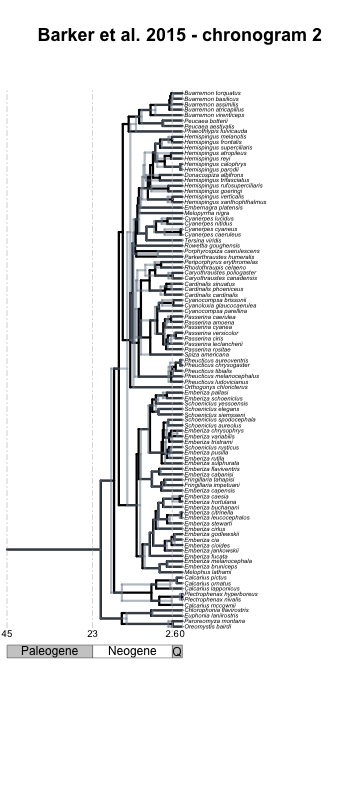
\includegraphics{../figures/figure-cross-validation/cross_validation_3.png}
\caption{Cross validation of Barker et al. (\protect\hyperlink{ref-barker2015new}{2015}) chronogram 1. The chronogram shown in black corresponds to the dates published in the original study. The gray chronogram corresponds to the same tree topology dated with BLADJ using node ages from all other source chronograms as secondary calibrations.}
\label{fig:cv3}
\end{figure}

\begin{figure}[!h]
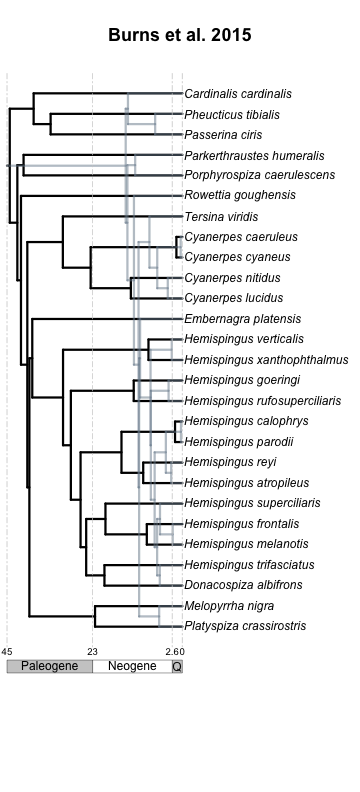
\includegraphics{../figures/figure-cross-validation/cross_validation_4.png}
\caption{Cross validation of Burns et al. (\protect\hyperlink{ref-burns2014phylogenetics}{2014}) chronogram. The chronogram shown in black corresponds to the dates published in the original study. The gray chronogram corresponds to the same tree topology dated with BLADJ using node ages from all other source chronograms as secondary calibrations.}
\label{fig:cv4}
\end{figure}

\begin{figure}[!h]
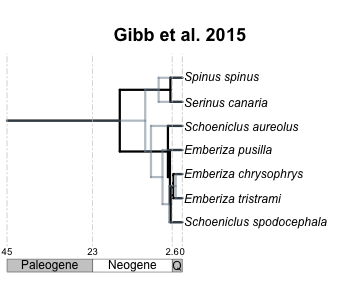
\includegraphics{../figures/figure-cross-validation/cross_validation_6.png}
\caption{Cross validation of Gibb et al. (\protect\hyperlink{ref-gibb2015new}{2015}), chronogram. The chronogram shown in black corresponds to the dates published in the original study. The gray chronogram corresponds to the same tree topology dated with BLADJ using node ages from all other source chronograms as secondary calibrations.}
\label{fig:cv6}
\end{figure}

\begin{figure}[!h]
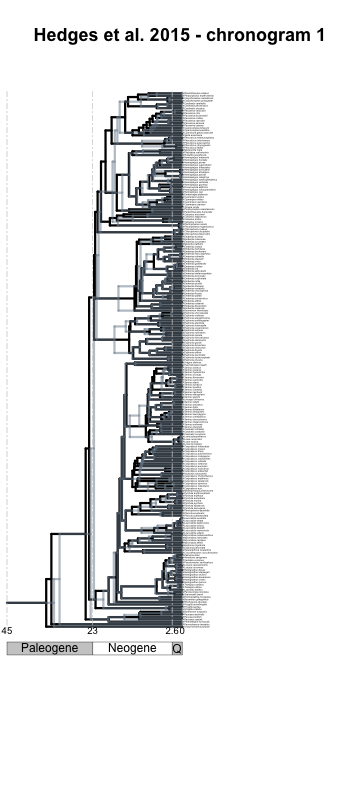
\includegraphics{../figures/figure-cross-validation/cross_validation_7.png}
\caption{Cross validation of Hedges et al. (\protect\hyperlink{ref-Hedges2015}{2015}) chronogram 1. The chronogram shown in black corresponds to the dates published in the original study. The gray chronogram corresponds to the same tree topology dated with BLADJ using node ages from all other source chronograms as secondary calibrations.}
\label{fig:cv7}
\end{figure}

\begin{figure}[!h]
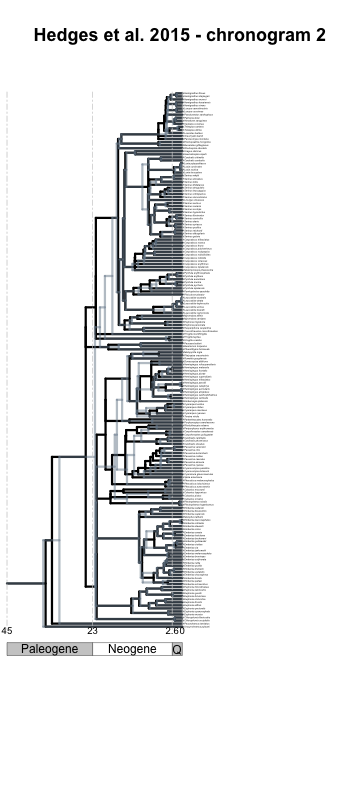
\includegraphics{../figures/figure-cross-validation/cross_validation_8.png}
\caption{Cross validation of Hedges et al. (\protect\hyperlink{ref-Hedges2015}{2015}) chronogram 2. The chronogram shown in black corresponds to the dates published in the original study. The gray chronogram corresponds to the same tree topology dated with BLADJ using node ages from all other source chronograms as secondary calibrations.}
\label{fig:cv8}
\end{figure}

\begin{figure}[!h]
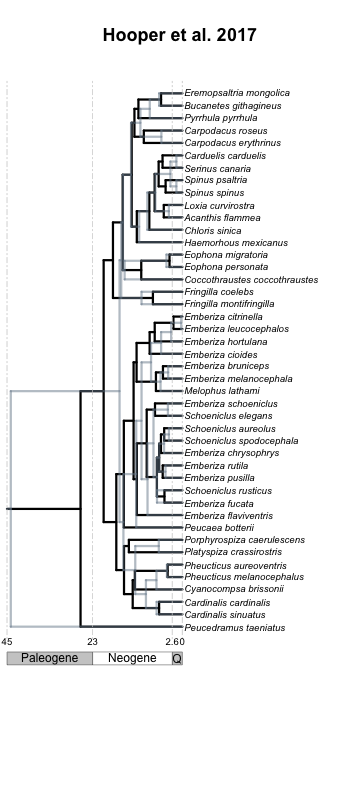
\includegraphics{../figures/figure-cross-validation/cross_validation_9.png}
\caption{Cross validation of Hooper and Price (\protect\hyperlink{ref-hooper2017chromosomal}{2017}) chronogram. The chronogram shown in black corresponds to the dates published in the original study. The gray chronogram corresponds to the same tree topology dated with BLADJ using node ages from all other source chronograms as secondary calibrations.}
\label{fig:cv9}
\end{figure}

\begin{figure}[!h]
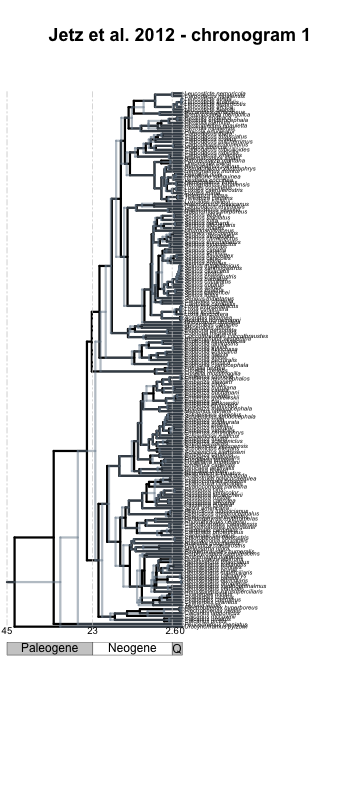
\includegraphics{../figures/figure-cross-validation/cross_validation_10.png}
\caption{Cross validation of Jetz et al. (\protect\hyperlink{ref-Jetz2012}{2012}) chronogram 1. The chronogram shown in black corresponds to the dates published in the original study. The gray chronogram corresponds to the same tree topology dated with BLADJ using node ages from all other source chronograms as secondary calibrations.}
\label{fig:cv10}
\end{figure}
